\chapter{General problem description}

Indoor tracking is a very complex matter, because the common GPS system is unavailable due to the fact that satellite signals are often absent or very imprecise inside buildings. From that very fact came the need to research other resources that could locate a user. In fact, many research labs and companies are developing solutions based on triangulation of Wi-Fi signals although this kind of systems are too imprecise\cite{wifiimprecise} for our purpose. 
Examples of problems with the triangulation are: signal loss, latency, continuous connecting and disconnecting from a range of Wi-Fi hotspots in order to measure the signal intensity. Moreover, a wireless solution will impact the autonomy of the device and the installation of Wi-Fi repetitors might be a burden for the final user. 
A marker, which is basically a symbol, avoids all those problems, although it brings another level of complexity by introducing other matters, such as: symbol recognition, data reading , quantity of information that can be stored, where it can be placed, etc.
There are several computer readable markers available on the market and the team decided to make a comparison between them before choosing one.
In fact, an RFID based solution has been produced and tested with simulation and experiments on the field.
This solution made use of a carpet composed by RFID passive tags which contained an id corresponding to a position saved on a local map. Furthermore, whenever the rollator with the RFID reader steps upon a tag it recognize the associated id and look for it into its database for the exact user's position. However, the current hardware implementation of an RFID reader doesn't allow any calculation on the trajectory of the walker, which is a necessary information for our purpose.The lack of this knowledge could be mitigated with other external resources but the solution proposed is not affected by this problem. Moreover, the results of the above mentioned study aren't ready to be published yet, therefore I can not compare the performance of this method with the one explained in this thesis.
 


\section{QRCode quick generalities}

A QRCode is an image containing an encoded binary matrix of data which looks similar to the one in figure \ref{qr} and it allows the storage of alphanumerical, numerical only, binary and kanji kind of information.
This markers are patented by DENSO WAVE INCORPORATED, which invented them, but the company choose to not exercise its right.
Therefore, QRCodes are largely used in many applications because they come free of any license and they are released as an ISO standard.

\begin{figure}[hbt]
    \centering
    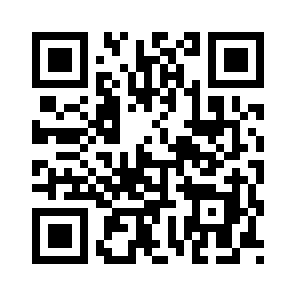
\includegraphics[scale=0.5]{img/qr.png}
    \caption{A generic QrCode. \label{qr}}
\end{figure}

It is composed by three bigger squares that indicates the position and it might have up to six other smaller squares which helps with the alignment. The basic unit composing the matrix is called module which is the tiniest black area that you can observe. There are 41 versions of it and they differ from each other by an increment of four modules. In fact, every matrix length is fixed and ranges accordingly to the version, from a minimum of 21x21 modules to a maximum of 177x177 modules. The algorithm used to encode offers the opportunity of error correction through the Reed-Solomon technique.\footnote{ according to: \url{http://raidenii.net/files/datasheets/misc/qr_code.pdf}}
Furthermore, because error correction needs to store those codes inside the matrix, the QRcode specification lists four level of correction capabilities: L, M, Q, H which respectively can restore 7, 15, 25 and 30 percent of data according to their codes length\cite{qrerror}.
The QRCode maximum capacity is obtained when using the 40 version combined with an L correction level, which offers the possibility to store up to 4,296 alphanumerical characters\cite{qrversions}.
Usually, programs which generates QRCodes chooses the right version and error correction level accordingly to the data's size which needs to be stored.

\newpage
To simplify what was explained in the earlier paragraph the following table shows a subset of QRCode versions, error correction level and the available space in bits for the user\footnote{complete table at: \protect\url{http://www.qrcode.com/en/about/version.html}}.

\vspace{2.5cm}
\begin{figure}[hbt]
    \centering
    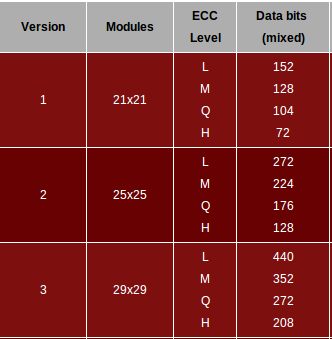
\includegraphics[scale=0.95]{img/qrversion.png}
    \caption{A partial table containing a subset of QRCode versions. \label{qrversion}}
\end{figure}

\newpage

\section{How QRCodes are used inside the thesis}

The proposed rollator has been instrumented with a camera connected to a processing unit which is empowered with a software for QR recognition.
All QRCodes contain a number (id) which identify unequivocally that exact location inside the building. In fact, the environment where the system has to work, must be analyzed in order to find spots where QRCodes can be put.
Usually, a good point where to place a tag is on the entrance of a room or after a cross, when the user begins to walk down a corridor. However, those general rules can be integrated with other necessity due to environments architecture. 
When all QRCode's positions are defined, a map containing all of them associated with the above mentioned id must be saved inside the processing unit.\newline
No methods to store this information is analyzed in this thesis, which assumes that the map is already saved. However, there could be many solutions for this problem, such as a QRCode at the beginning of a floor containing its map or maybe that this database is transfered via bluetooth or even pre-downloaded at home before the arrival. No methods of QRCode's encoding is analyzed neither, because there is plenty of software available to the public which generates the needed image.
\newline
However, the proposed algorithm's role is to look for QRCodes inside a picture, read it and compute the QR's angle relative to the camera. Moreover, the rollator on which I worked on has an estimation of the trajectory calculated with odometry techniques. Therefore, the angle found with the algorithm is used to reduce the approximation of the trajectory and diminish ,also, the error given by the system to a future application with step by step directions. In addition, this method allows to better know the position inside the gap between two markers.






   













  
